\chapter{Approach}

In this section, I present the design of my replacement for the original Project EPIC infrastructure. As mentioned above, my design relies on a microservices architecture that is deployed on a cloud-based infrastructure making use of container orchestrated technologies to coordinate all services and deploy them in a distributed fashion. Thanks to this design, I am able to use fewer physical machines while optimizing the computational power I have available.

For the system description, I will use a comparison with the previous existing Project EPIC infrastructure, comparing each component with the new proposed infrastructure. First, I will discuss the collection architecture and its persistence layer. Then I will describe the analysis infrastructure and I will end by describing my user interface layer and comparing it with EPIC Analyze.

\section{Data Collection and Persistence}

\subsection{Previous infrastructure}

\begin{figure}[htbp]
	\caption{\label{fig:oldinfrcollection}
	Diagram highlighting the data collection parts in the old infrastructure.
	}
    \begin{center}
	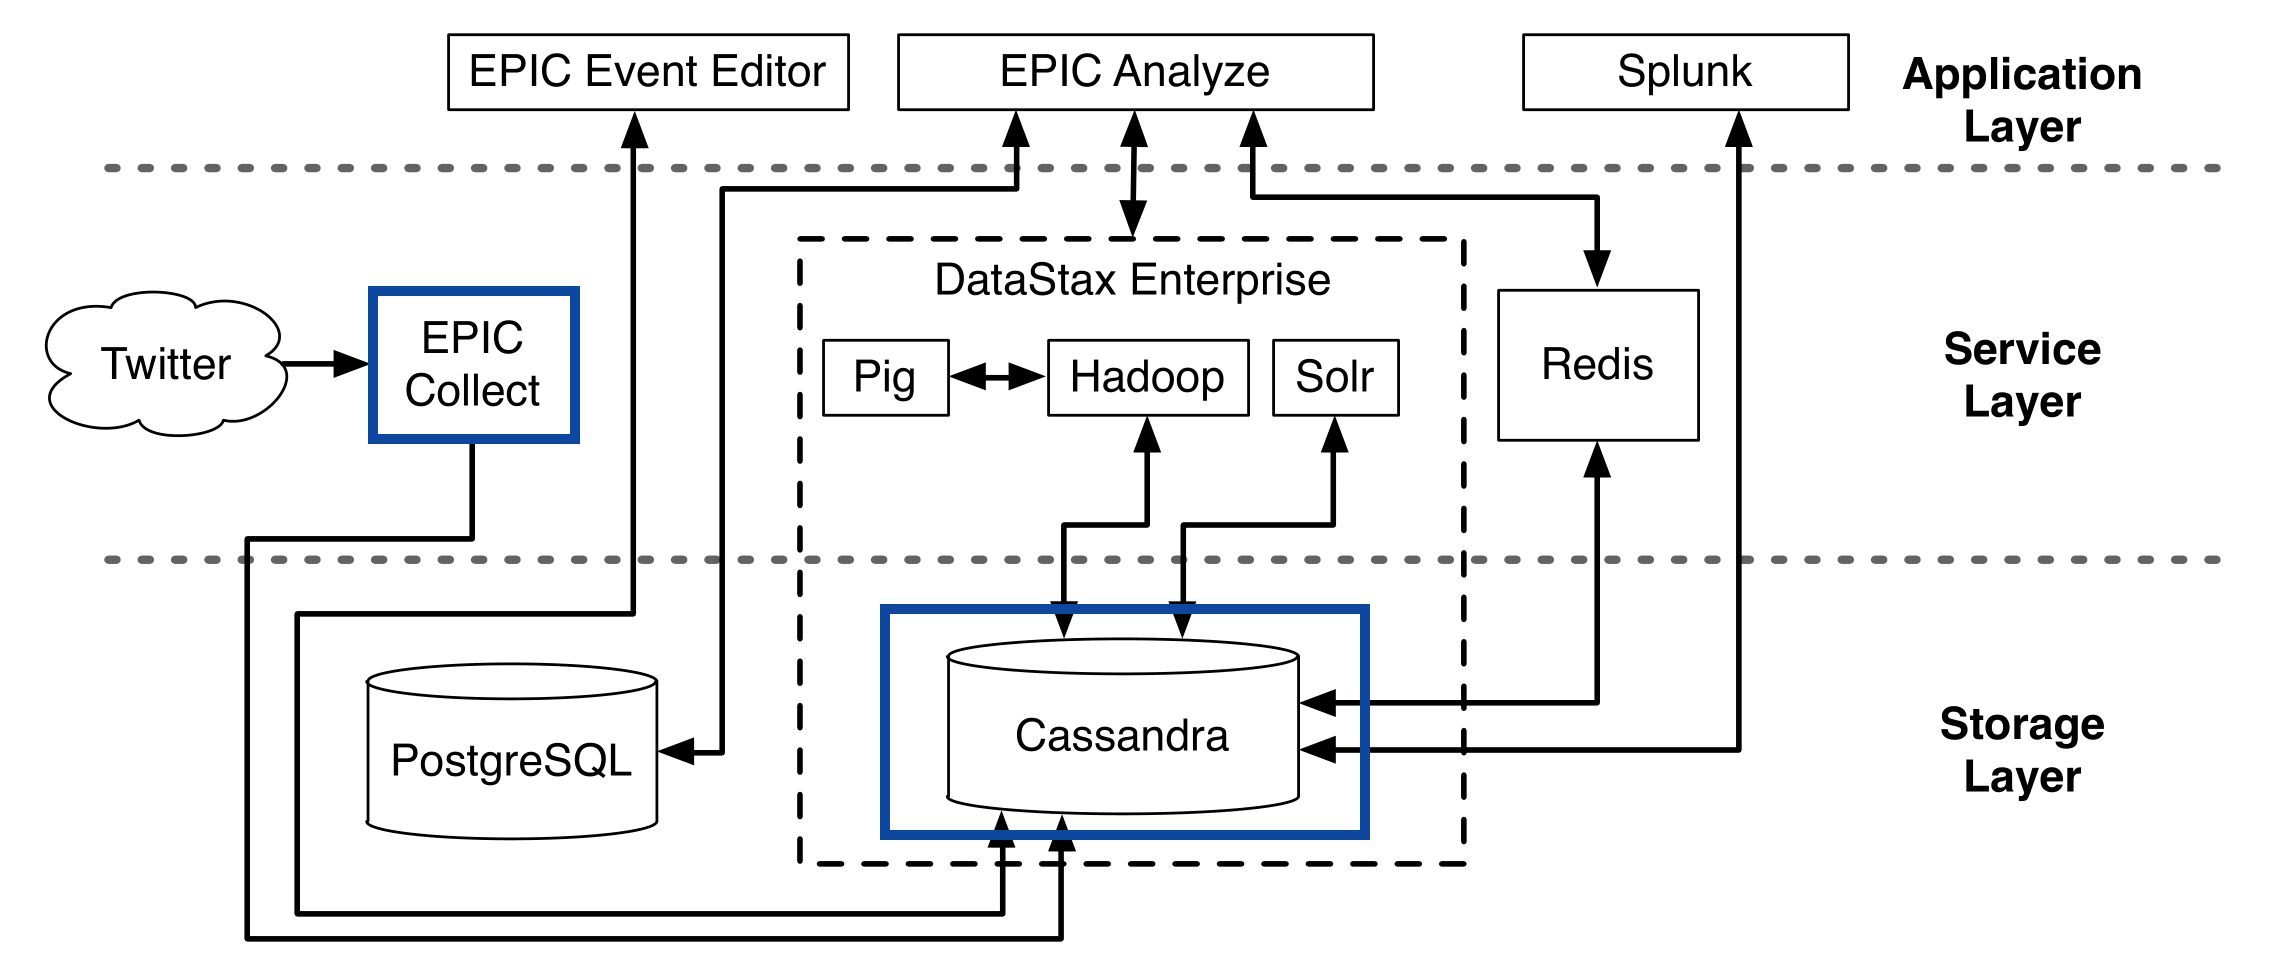
\includegraphics[width=150mm]{figs/old-arch-collection.png}
    \end{center}
\label{xfigDiagram}
\end{figure}

Data collection in the previous infrastructure is mostly composed by the monolithic EPIC Collect. The system is designed to be composable within itself by using the Spring framework to do dependency injection between different services. To collect tweets, it connects to Twitter’s Streaming API directly. It uses a separate thread to monitor the keywords needed and restarts the collection thread when the keywords are updated. Those keywords are updated through the EPIC Event Editor. This web application allows users to create and stop events and their associated keywords. Updates via this web application changes fields in the EPIC Collect database; these changes are then detected by the EPIC Collect thread which restarts its collection to make use of the new keywords. 

To process the tweets and separate them into events, the system keeps an in-memory queue that separates the ingestion part of the infrastructure from the classification component. The classification mechanism checks events tracked at the moment and classifies tweets to the events it matches. This process, once finished, sends tweets to the persistence layer. 

Data was stored first in MySQL and then in Cassandra. Project EPIC researchers were forced to switch to Cassandra after realizing that using MySQL created a bottleneck when storing tweets. In addition, to process data faster, there is a need for data to be distributed across multiple machines to increase parallelization and allow real-time computation. Data is stored using the event id as the key. This allows retrieving tweets by event faster. In addition, to allow for quick date range queries, it includes the day in the key such that time-slicing queries are fast. The design of the key also helps to balance data evenly across the Cassandra cluster \cite{anderson2015design}. 

\subsection{New infrastructure}

\begin{figure}[htbp]
	\caption{\label{fig:newinfracollection}
	Diagram highlighting the data collection parts in the new infrastructure.
	}
    \begin{center}
	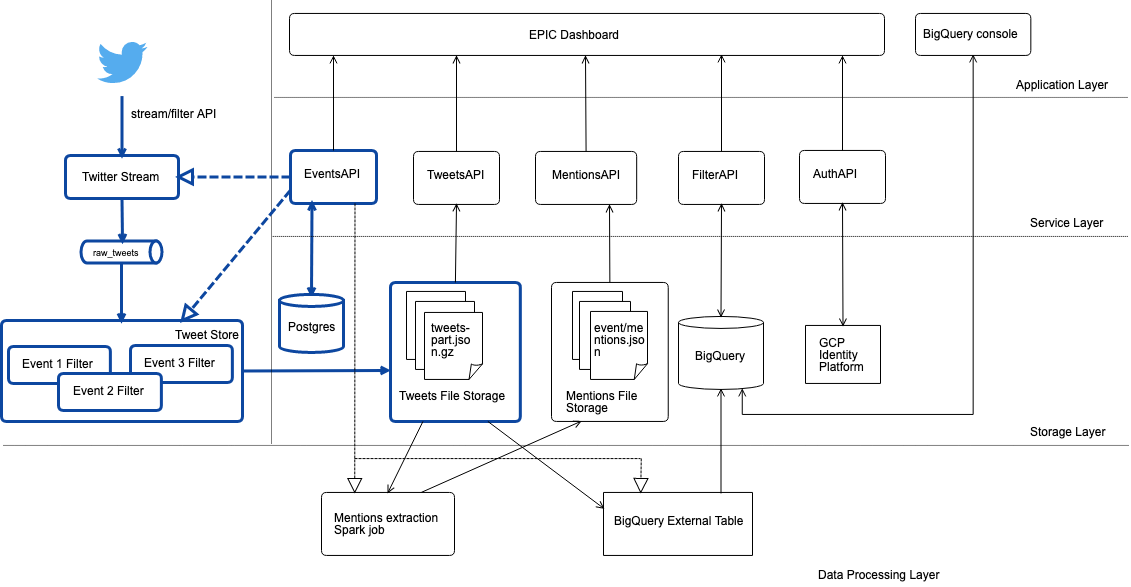
\includegraphics[width=150mm]{figs/infrav1_collection.png}
    \end{center}
\label{xfigDiagram}
\end{figure}

In order to make collection faster, I designed the collection components to be stateless. That is, these components are designed to perform operations based only on the messages they receive. This makes the system more reliable as it allows the underlying container orchestration system to replace crashed services and scale up if needed. 

Data collection from the API needs to be really reliable. It also needs to be available to ingest multiple events at the same time. One of the main concerns with this part of the infrastructure was how to avoid losing messages at peak times while avoiding having a huge infrastructure running all the time. For this, I designed the ingestion pipeline to use Kafka between stages so that it can cache messages during peak times and process them all at once after the rate of messages decreases. It also acts as another reliable mechanism that can help crashed services recover non-processed messages once they are back up. This acts similarly to the in-memory queue from the old infrastructure but is more reliable. I separated the pipeline into two services: ingestion and filtering.

For ingestion, there is the Twitter stream connector. Its function is to connect to the Twitter Streaming API using a defined set of keywords and send incoming messages to Kafka. The set of keywords are pulled from a Configuration Map in Kubernetes. This service is periodically checking a local file with the keywords to restart the collection if they change. Thanks to the microservice approach, I was able to leverage the Go language for this microservice instead of Java. This is because I needed increased reliability and good message processing capabilities. Go provides a good network interface and allows for quick message processing. Note that this service does not process tweets in any way, it only retrieves them and sends them down the pipeline to Kafka. 

The next step in the pipeline is the filter service. This service is fully stateless, it relies only on the messages in Kafka. In addition, each service instance is event specific. The system only runs an instance of the filter service for each event active at any given time.  If no active event is being tracked, there are no filter instances running, which means that it is only using computing resources when needed, allowing us to use more resources for analysis. 

For reliability, when an instance goes down, it reconnects to the latest offset committed to Kafka. I use consumer groups from Kafka to distinguish between different filter services reading at the same time from the same topic. Once a tweet arrives at the filter service,  the service decides whether or not it belongs to the current event. It does so by doing a simple string search on the tweet JSON. If any of the keywords from the event are in the JSON, that tweet is classified as pertaining to the event and buffered. 

To store tweets, I rely on a cloud object storage service. This service serves as an online file system, abstracting away data distribution and replication. This allows me to work under the contract of reliability from the cloud provider and forget about implementing reliability measures like data replication. In addition, thanks to the availability of long term storage options, I can keep data storage costs low. I have programmed the data to fall into cold storage after a year, allowing the infrastructure to retrieve the data faster while it is being collected, and reduce costs after a year has passed since the need for that data is likely greatly reduced at that point.

The filter service is in charge of uploading tweets to the object storage service. Every hour, the service compresses all messages in its buffer and uploads them to the object storage service as a single file. To handle peak usage times while ensuring good performance for analysis, the service will also upload messages if the buffer fills to 1000 tweets. 

To provide fast querying of tweets given an event and to provide support for time slicing queries, I use the file system abstraction to store  metadata on the filename and path. On one hand, I store each file into their corresponding event folder. This allows listing all files with tweets for a specific event fast, as it is only listing all files under a folder. On the other hand, I store the date and the number of tweets in a file in its filename. Thanks to this design, I can later parse the filename and detect if I have any tweets that I need in the file. File names thus work similarly to an index. I keep the number of files low by setting the buffer size limit high. Thanks to this index, I also can create a visualization of ingestion rate per hour without needing to access the files. 

Organizing all this, I developed the Events API. This service is in charge of performing CRUD operations to events. It uses a PostgreSQL database to store the events data and their status. It also keeps track of when an event collection is started or stopped, and which user is responsible for the action. This service is also in charge of updating the pipeline described above if needed. This service interacts with Kubernetes to instantiate new filter services when an event is created or a collection is restarted. It also manages the configuration map that maintains the set of keywords to be collected at any given point in time. This service is in charge of abstracting all event-related actions. It exposes a REST interface used by the infrastructure's user interface.

\section{Data Analysis}

\subsection{Previous infrastructure}

\begin{figure}[htbp]
	\caption{\label{fig:oldinfaranalysis}
	Diagram highlighting the data analysis parts in the old infrastructure.
	}
    \begin{center}
	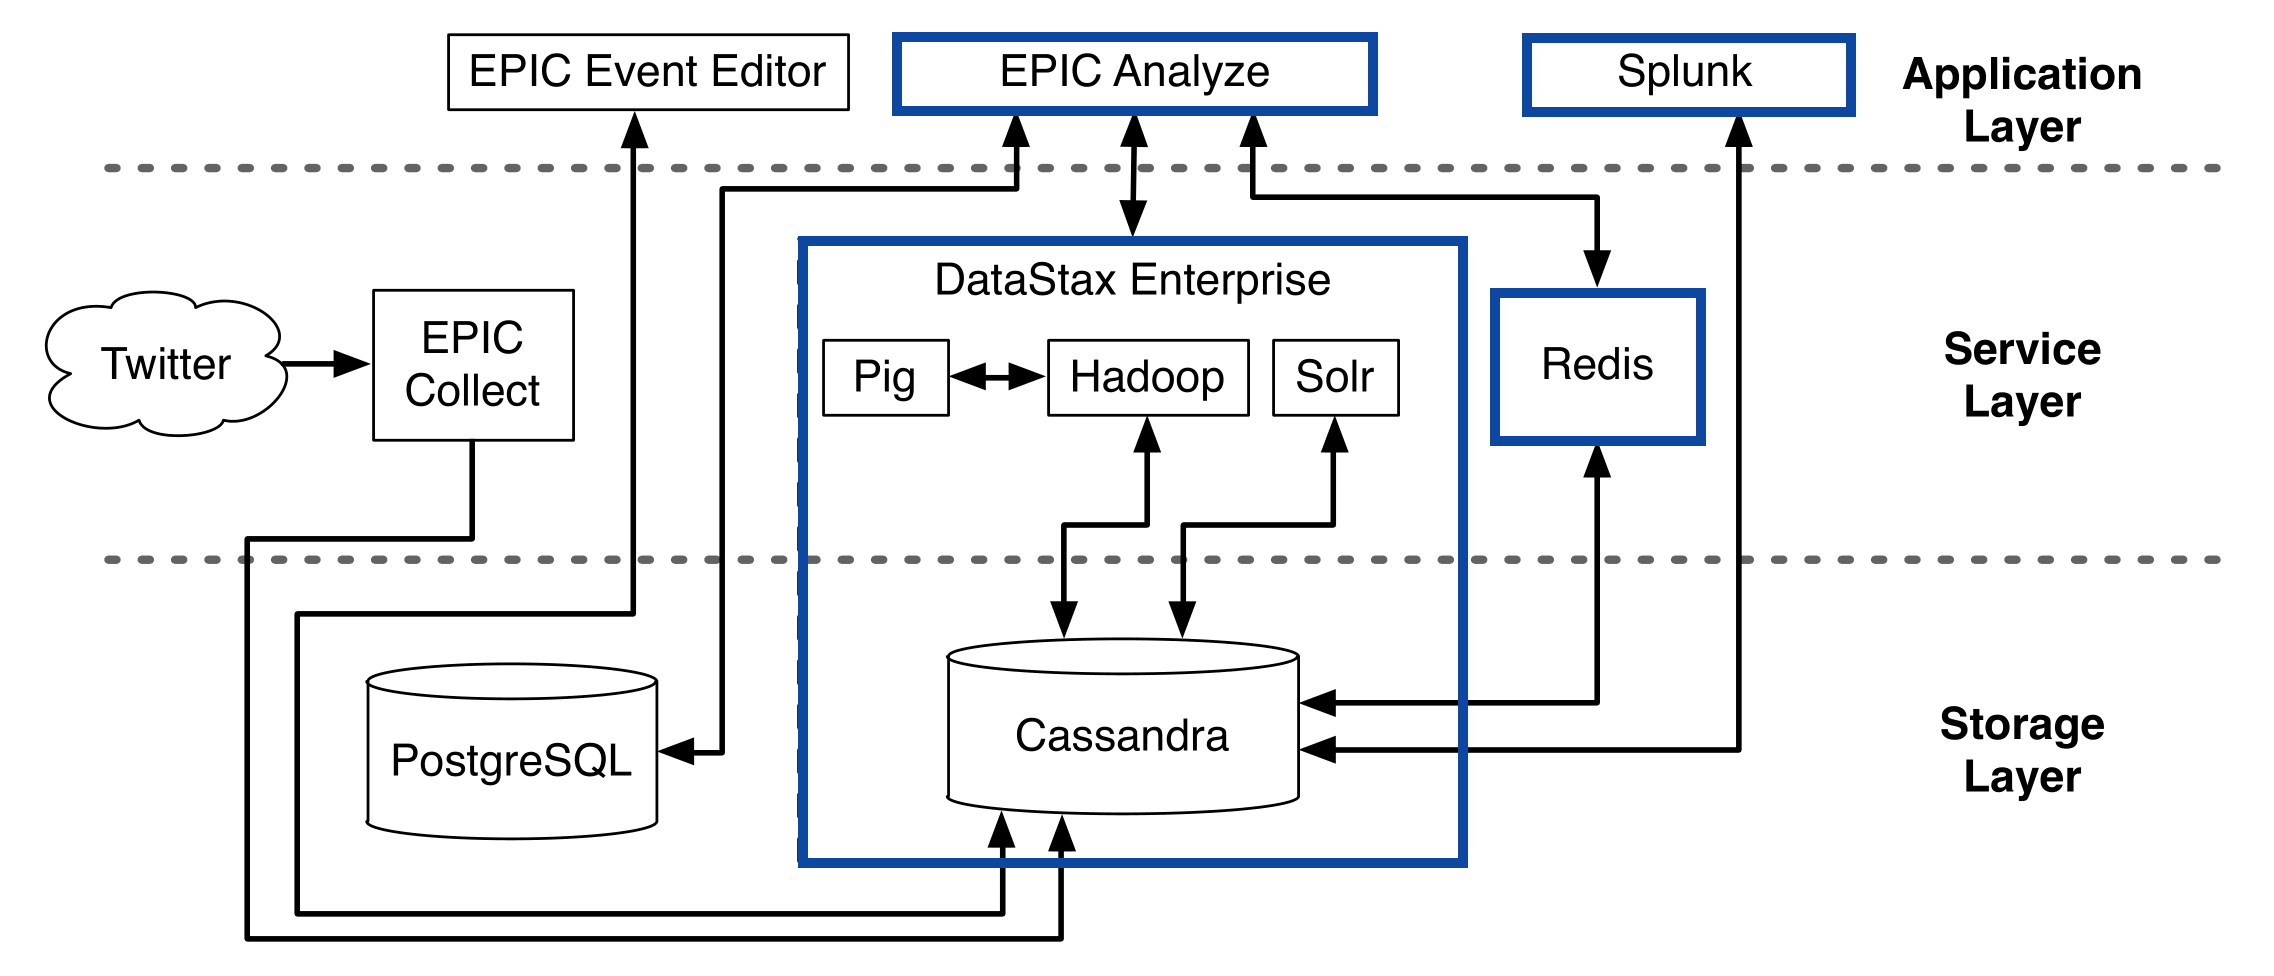
\includegraphics[width=150mm]{figs/old-arch-analysis.png}
    \end{center}
\label{xfigDiagram}
\end{figure}


Previous work on Project EPIC on data analysis is presented across several papers. First most work started as a SQL query when data was still stored in MySQL. Due to the switch to NoSQL technologies for storage, the technical difficulty to access collected data increased. This, in turn, made it complicated to filter data sets and explore them. To address this situation, software engineers had to interact with analysts to narrow down data sets and expose them in a format that would be easy for them to import into third-party tools. This was a highly manual process. 

To improve that process, EPIC Analyze was created. This monolithic system used a model of data sets associated with events to load and visualize the data. Due to Cassandra not being good at supporting random accesses and the main cluster needing to be available for peak ingestion times, the analysis needed to happen in a separate cluster. EPIC Analyze had its own Cassandra cluster where data sets to be analyzed were stored. The process of loading the data to be analyzed was done manually. The main functionality available in EPIC Analyze was browsing and pagination, filtering, and the job framework.

For browsing and pagination, EPIC Analyze allowed exploring the data set at the tweet granularity level. It paginated the data using Redis indexes created when data was imported to the system. Each entry in the index pointed at the column and key where a tweet was in Cassandra. Thanks to Redis, pagination was fast. This allowed analysts to interact with each other by finding important tweets and sharing pages where interesting tweets were located.

Filtering was aimed at reducing the size of the data to be explored. EPIC Analyze allowed analysts to specify a search query based on various fields from a tweet. This took advantage of the DataStax Enterprise integrated version of Apache Solr with Cassandra. Solr built indexes when data was loaded into the analysis cluster, allowing for sub-second queries when the index was finished.

Finally, for other analysis techniques, EPIC Analyze had a job framework available to extend the capabilities. This framework used Resque to queue jobs and perform them. Some of those jobs used the Apache Pig QL language to query the dataset for deeper insights. Output results were stored in Cassandra in the form of JSON. This was accessed by EPIC Analyze and showed in the UI either in RAW form or in visualizations if implemented.

A limitation on this design is the fact that data needed to be transferred to a separate cluster for analysis; this made the job of analyzing the data set asynchronous to the event itself. This can be dangerous, as analysts are blind to what is happening in an event until the event is loaded into EPIC Analyze. In addition, even though Datastax does a great job at integrating Hadoop with Cassandra, performance is hugely influenced by what is happening in the Cassandra cluster. This means that two MapReduce jobs running on separate clusters will find a bottleneck when they try to read from Cassandra at the same time, as the cluster will need to perform both reads simultaneously. This is similar to an issue I encountered with the infrastructure proposed in my undergraduate thesis. There Spark had issues loading data to memory while Cassandra was collecting data since Cassandra was running out of memory.

\subsection{New infrastructure}

\begin{figure}[htbp]
	\caption{\label{fig:newinfraanalysis}
	Diagram highlighting the data analysis parts in the new infrastructure.
	}
    \begin{center}
	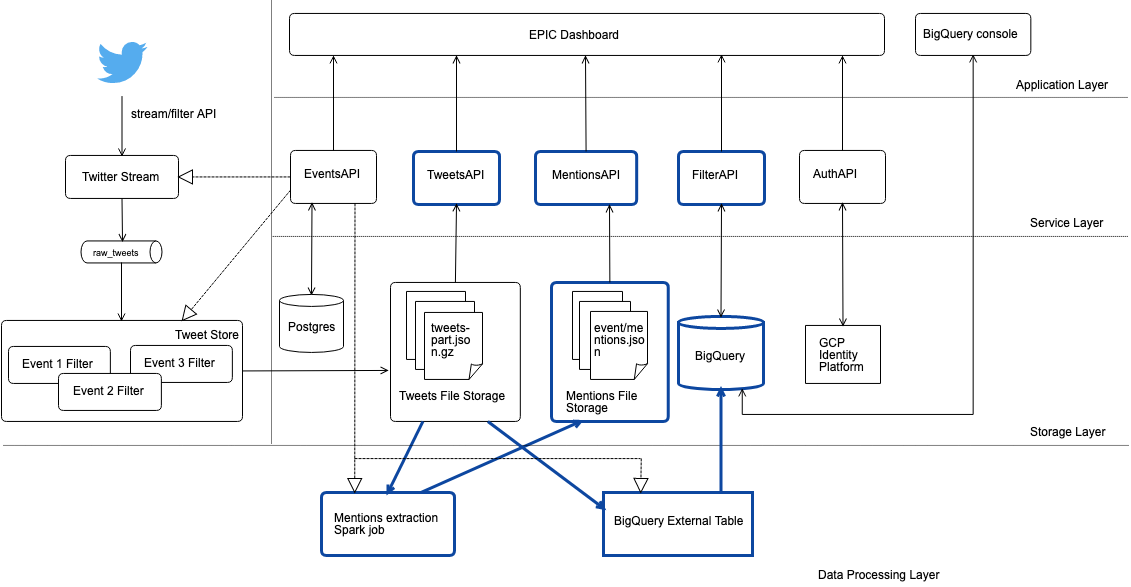
\includegraphics[width=150mm]{figs/infrav1_analysis.png}
    \end{center}
\label{xfigDiagram}
\end{figure}

As previously discussed, there is a need to explore and analyze collected disaster data sets in a way that analysts can understand what people were discussing during the event. On one hand, my infrastructure needs to allow users to scroll through an entire data set with ease, abstracting the underlying storage layer. On the other hand, I want to provide a way to query the data set with a high-level language like SQL for interactive exploration of the data set. This would allow analysts to test theories and understand the data set at a deeper level than what browsing provides. In addition, my system needs to be able to do some analysis in batch mode after finishing a collection to help load an event's data more quickly into the user interface.

For data exploration, I built the Tweets API. This microservice abstracts the underlying data storage layer. It uses the filenames with tweet counts to create a pagination index. This index is used to calculate what file is needed to retrieve particular tweets. This file is calculated from the index given a page number and the number of tweets per page. This index can be created given a list of all the files under an event's directory. Due to Google Cloud Storage API’s being slow when the number of files to list starts to exceed a certain size, I decided to cache the index in the memory of the Tweets API microservice for 10 minutes. This allows analysts to quickly explore data sets, being able to load any page in seconds. Thanks to this API, I abstract away the storage layer from the user interface. In addition, as the event name is passed as a variable, this API is completely independent of the Events API. This follows the software engineering rule of reducing dependencies as much as possible. In addition, it also allows for performance patches to be deployed on the exploration part of the infrastructure independently from the collection-related components.

Similar to EPIC Analyze, I also added the ability to annotate tweets. Analysts can add arbitrary tags to tweets in a data set. These tags are color encoded using a hash function based on the text to enable fast visual exploration. These annotations are stored in PostgreSQL using the Events API.

Another factor that takes importance is time slicing during data exploration. Using the date on the filename, I can filter what part of the pagination index I want to use. This can be done in linear time. After the filtering has happened, I can calculate again what file to retrieve.

For filtering, I rely on Google Cloud BigQuery service. This service allows me to query the dataset in SQL interactively. I use the Filter API to abstract away the details of the interaction with BigQuery. This API returns data in a format similar to the Tweets API. The difference between the two is that the data returned is only the data needed for presenting an overview of a tweet. I did not implement all the filtering options that existed in EPIC Analyze, but I do know that the same functionality can be achieved over time. At the moment, I implemented only text search using the like operator on BigQuery. I use temporal tables to paginate through the results. To access details from a tweet, I provide the filename and tweet id to the Tweet API. That API can then retrieve the file and return the full tweet JSON to the user interface.

Thanks to BigQuery, I can also personalize and export data into CSV format on demand. Using SQL, I can narrow down the data set and choose the fields I want to expose. Once that is done, I can export the results into a CSV stored in Google Drive. This is especially useful for Project EPIC interactions with external collaborations.

For additional analysis jobs, I leverage Google Cloud Dataproc and Spark. I created a workflow template on Dataproc which gets triggered every time an event collection is stopped by the Events API. This workflow can be modified independently of the rest of the infrastructure by adding new Spark jobs. Jobs receive the event name as a parameter. Spark jobs are written in Java and stored in Google Cloud Storage as jar files. This jar is loaded on a cluster created when the workflow is triggered. Creating clusters on demand avoids having unnecessary servers sitting around when there are no analysis jobs running.

The first Spark job added is the mentions extraction job. I believe that extracting the most mentioned users from a data set can lead us to find the most important users in a data set. This information can be later used to extract their timelines and contextualize the collection further. 

Developers must also create APIs to expose the data that Spark jobs extract. In this case, there is a Mentions API that knows how to access the resulting output from Spark and serve it in a paginated fashion. 

Note that adding a new batch job does not need any interaction with the rest of the services. This allows for new developers to work on extensions without any need to change existing services. The only step needed to interact with other code is the user interface; I will that component in more detail below. In the mentions extraction case, to prove that this was a good approach for parallel development, it was developed on the side of the rest of the infrastructure by a different developer. This developer worked by himself to create this extension. The only part of the code base that he needed to change in my system was within the user interface. This provides a powerful way to extend the capabilities of the system in the future.

\section{User Interface}

\subsection{Previous infrastructure}

\begin{figure}[htbp]
	\caption{\label{fig:oldinfrui}
	Diagram highlighting the user interface parts in the old infrastructure.
	}
    \begin{center}
	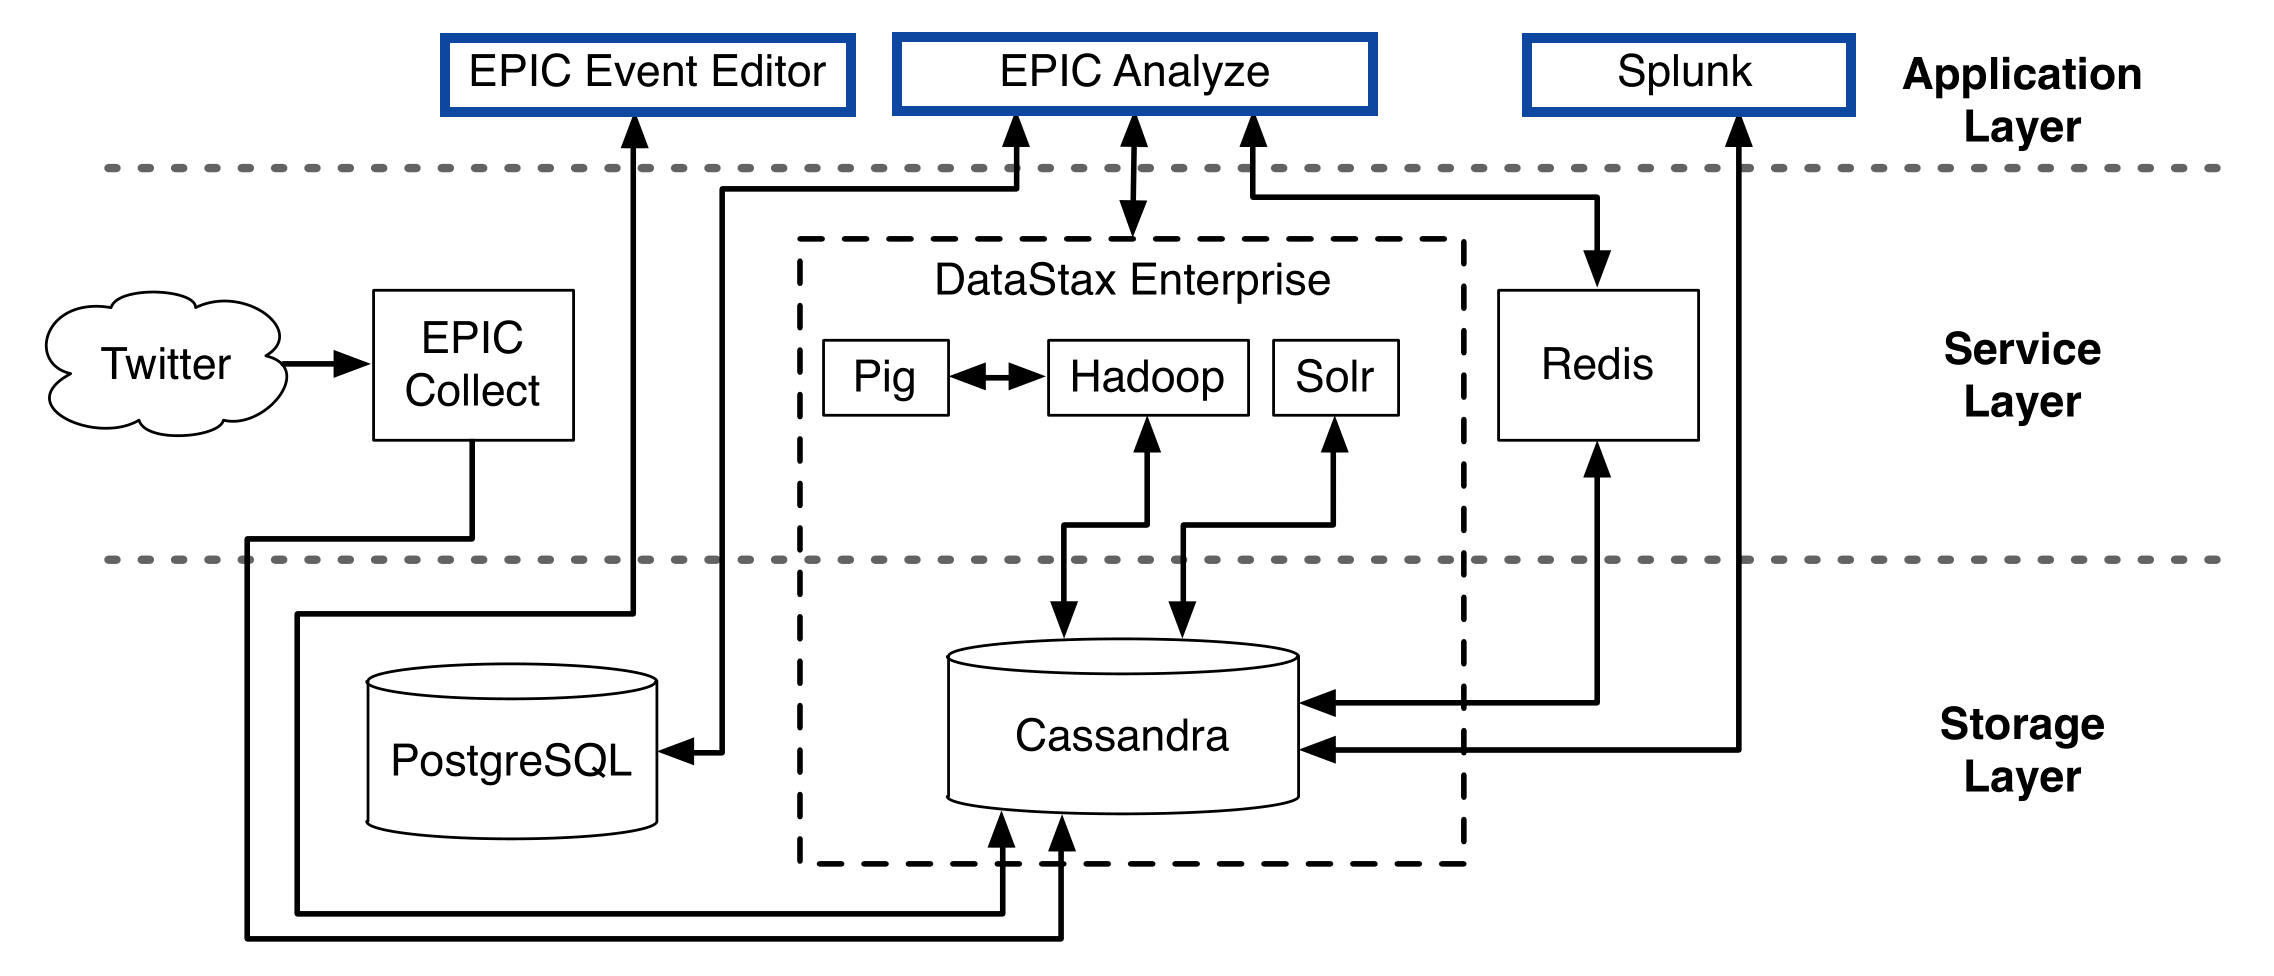
\includegraphics[width=150mm]{figs/old-arch-ui.png}
    \end{center}
\label{xfigDiagram}
\end{figure}

There have been several iterations on the user interface for EPIC. The latest was developed as part of EPIC Analyze. This monolithic app is built on Ruby on Rails. Coupled with Redis and Cassandra, it provided an interface for data set interactive exploration. The interface was done in the form of a web app. Designed with Ruby on Rails views, the code was highly coupled to the underlying infrastructure. This meant that to add new capabilities to the existing user interface, developers needed to expand on the already existing application, creating a highly coupled system that increased in complexity over time. 

Focusing on the web application, we can find a list and detail view to explore tweets in a data set. Tweets can be explored page by page in the browser, and each tweet can be expanded to see all of its related metadata. On top of the page there is a timeline that shows the volume of tweets over time for the existing data set. The analyst is allowed to select a period of time by drag-and-drop interaction on the timeline, allowing for the data set to be time sliced. EPIC Analyze also provides a querying interface to perform complex queries with composed conditions. This functionality allows for analysts to filter down datasets by different elements from the tweet metadata. These queries also update the count timeline to reflect the tweet volume of the new filtered data set.

Another interface element provided was the EPIC Event Editor. This was a simple user interface to associate keywords to events. This was plugged in to EPIC Collect to determine what tweets to retrieve for each event. From this interface you could start and stop collections at any given time. This system was completely independent from EPIC Analyze, as the later needed data to be loaded into manually to analyze it as discussed above. This requirement was due to the design of the previous infrastructure. 

Finally, the last element of the old user interface is Splunk. This is an application that manages and allows for queries to be written in a domain specific language on top of Cassandra. This allowed for real time queries. The main problem was that you needed to use the Splunk pipeline language to perform queries. Splunk was also completely independent from EPIC Analyze and the EPIC Event Editor interfaces.

On the user management aspect, EPIC Analyze exposed a set of abstractions to manage permissions and access to data sets. User affiliations restrained access to certain data sets. User accounts needed to be created on the Postgres database to support this. Splunk had its own authorization mechanisms as did the EPIC Event Editor, all independent from each other. 

\subsection{New infrastructure}

\begin{figure}[htbp]
	\caption{\label{fig:newinfrui}
	Diagram highlighting the user interface parts in the new infrastructure.
	}
    \begin{center}
	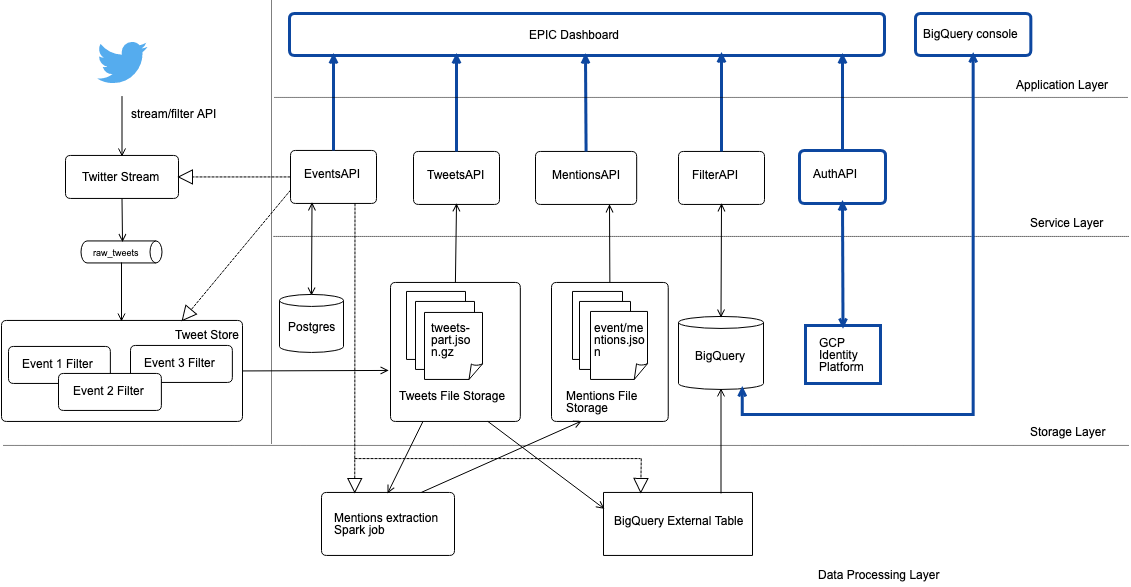
\includegraphics[width=150mm]{figs/infrav1_ui.png}
    \end{center}
\label{xfigDiagram}
\end{figure}

For the new infrastructure, I looked for a front-end framework that would be able to modularize each user interface element independently. The main reason behind this decision was to allow for various developers to work on interfaces of their own APIs independently. There are many frameworks available to develop front end applications. My goal was to find one which is suitable for building real-time dashboards. 

According to a study, the most popular front end frameworks are React JS, Vue JS, and Angular JS. Upon more research, in 2019, 78.1\% of front end developers use react, 0.8\% use Vue and 21\% use Angular. The clear winner in terms of frameworks that I wanted to use was React JS. React JS also breaks down its pages into components, each of which can be developed in parallel. The way React works is that when a component receives new data, only part of the page refreshes  which is exactly what I needed for my infrastructure's user interface. Each API in our dashboard can be treated as a smaller independent application. This separation needed a framework for application state management, that is a tool which is responsible to segregate functions and data. The best application framework out there to currently work seamlessly with React is Redux.

This approach to our user interface design allows teams to work in parallel on different elements from the user interface and compose it all on a single application app. With this approach, an API developer, can decide on their own data visualizations and integrate them into the rest of the user interface separately. In addition, the interface is more robust as it is fully independent of the back-end code and it only interacts with the JSON data representations exposed by the various APIs.

\begin{figure}[htbp]
	\caption{\label{fig:mentions}
	Most mentioned users in a dataset, ordered by number of mentions descending.
	}
    \begin{center}
	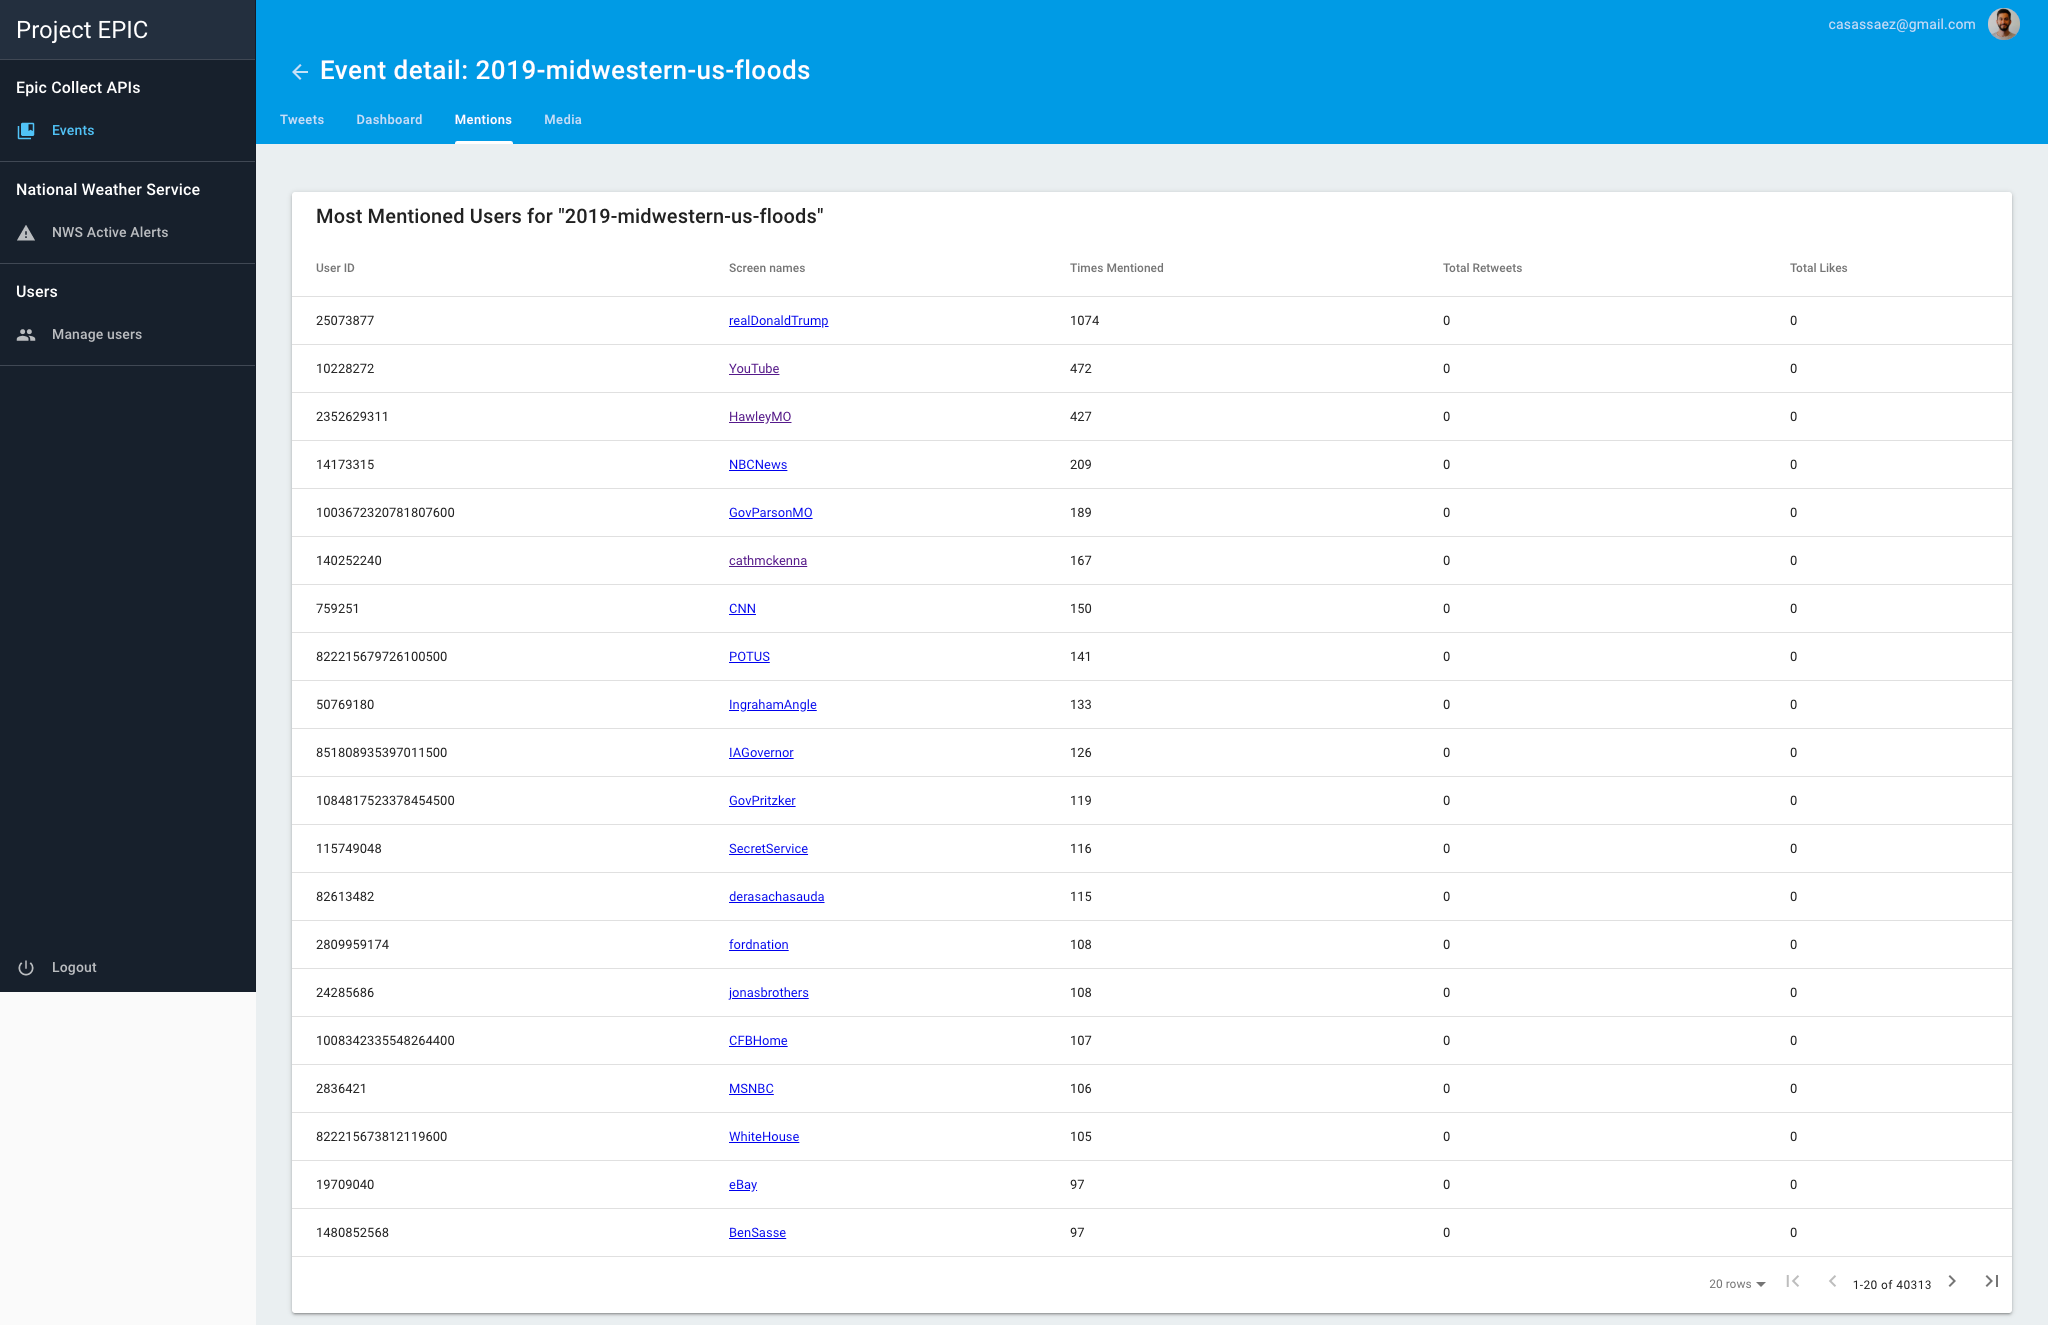
\includegraphics[width=150mm]{figs/mentions.png}
    \end{center}
\label{xfigDiagram}
\end{figure}

An example of such a component is the Mentions integration (see Figure \ref{fig:mentions}). It integrates the mentions from the events in a new tab from the events page. It was implemented separately and only the event name is sent to it. This allowed for development of the user interface in parallel with other aspects of the infrastructure.

\begin{figure}[htbp]
	\caption{\label{fig:tweetlist}
	Tweet list user interface in the new infrastructure.
	}
    \begin{center}
	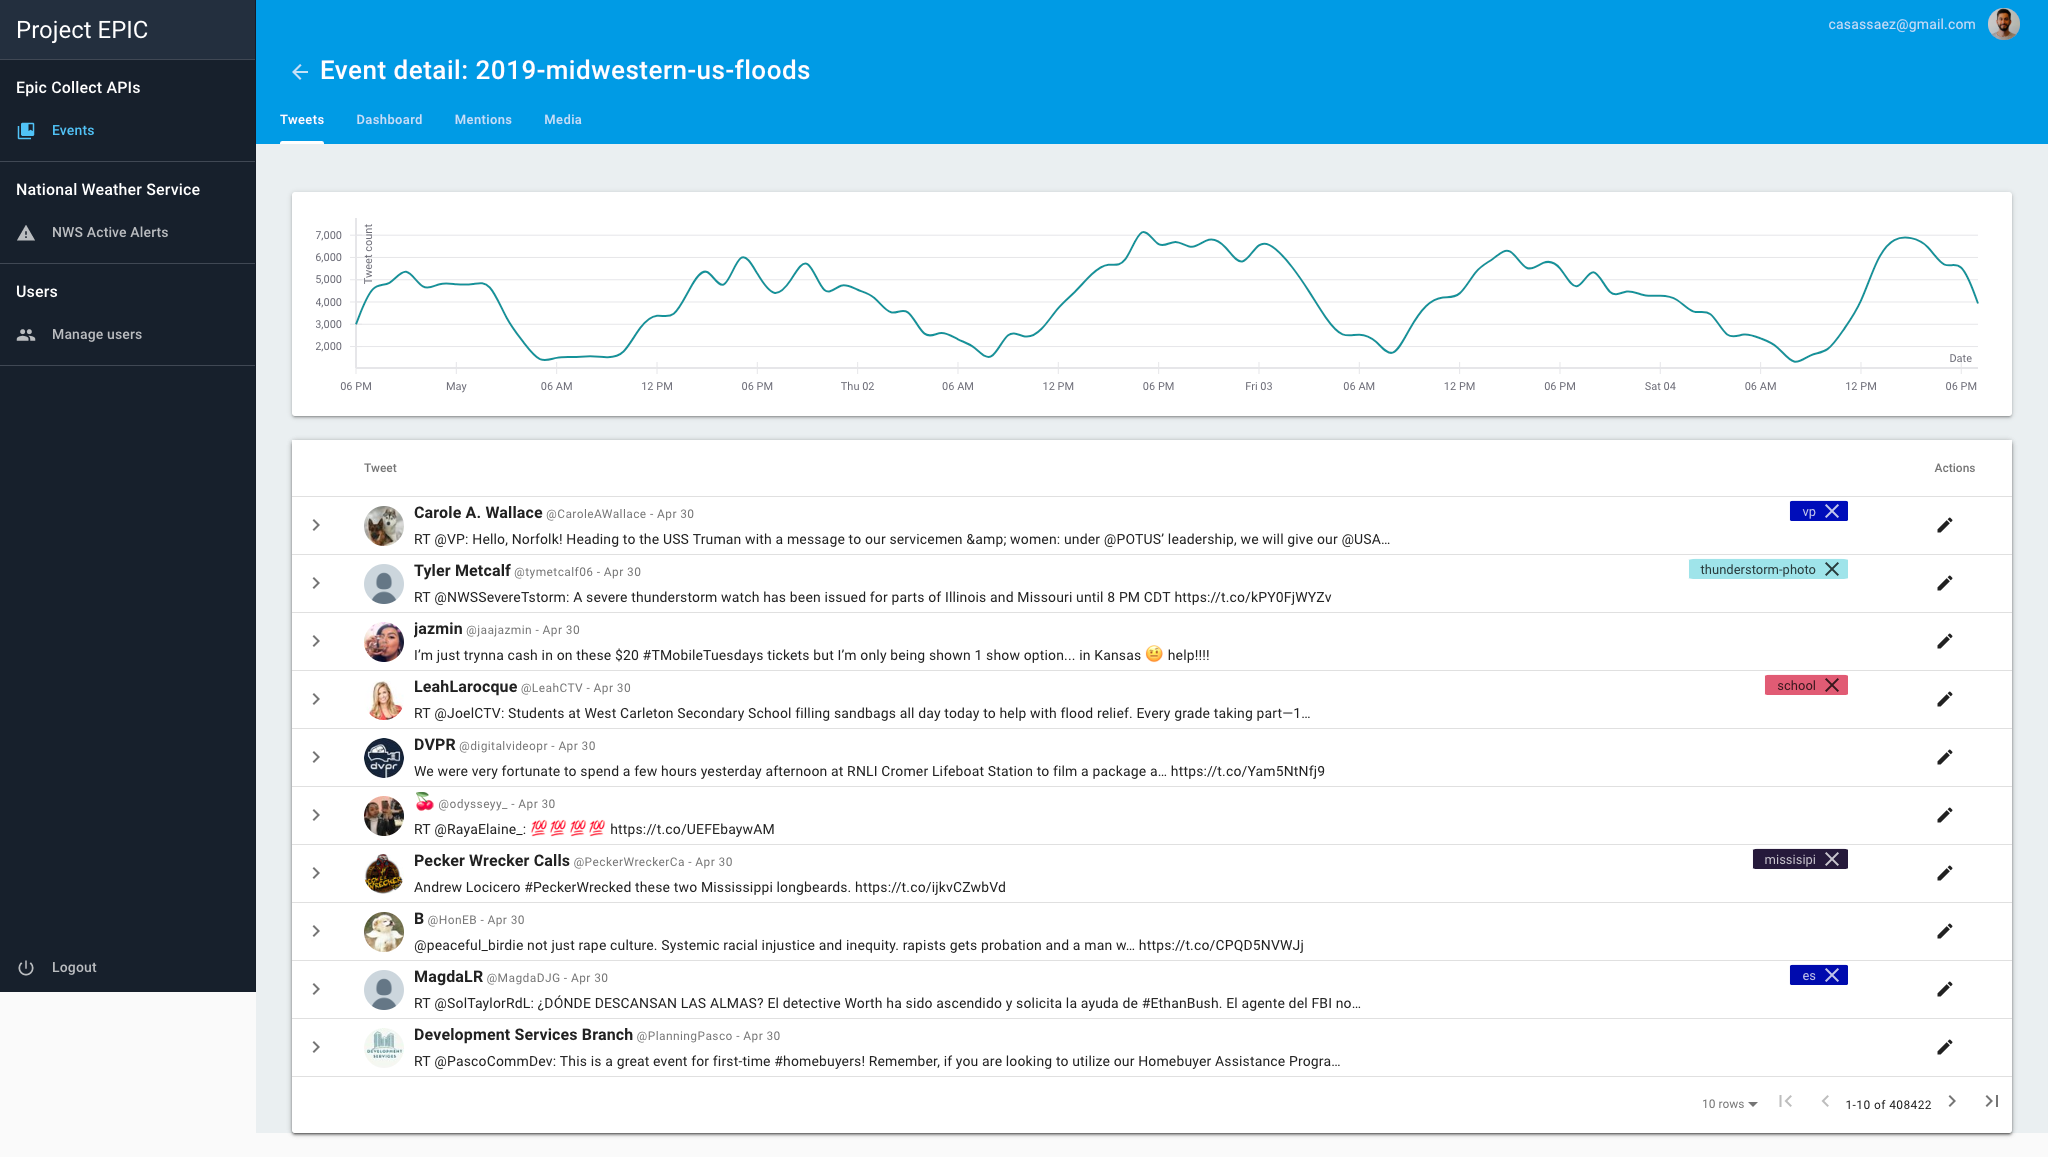
\includegraphics[width=150mm]{figs/tweet-list.png}
    \end{center}
\label{xfigDiagram}
\end{figure}

To explore events, an interface was created similar to the one described for EPIC Analyze \cite{barrenechea2015getting}. There is a list of tweets with a timeline visualization above for time slicing the data set (see Figure \ref{fig:tweetlist}). Each tweet can be expanded to explore all the metadata associated with it, similarly to the functionality in EPIC Analyze. In addition, thanks to its composability, the user interface can also integrate external APIs easily. An example of this is the incorporation of  National Weather Service alerts. Using their public REST API that provides all current alerts information, I created a visualization of the active alerts. This way, the user interface could act as good integration with an external API, avoiding inserting new dependencies in the back-end.

To allow more technical analysts to perform deeper analysis, the system also points to the internal BigQuery table in Google Cloud Console. This allows analysts to explore the data set in a more interactive way using Google BigQuery directly.

Finally, in order to simplify interaction with each internal API, an ingress gateway was created. This portal aggregates all APIs under the same IP allowing the frontend to work as if it is a single API. In reality, each API is independent of each other. This gateway works by establishing rules for forwarding traffic to the corresponding API. This ingress is created by Kubernetes and associated with a static external IP, to avoid IP changes between cluster restarts. I also added an SSL certificate to the gateway using Kubernetes managed certificate service. This helped secure the application. 

\subsubsection{User interface diagram}

\begin{figure}[htbp]
	\caption{\label{fig:frontdiag}
	EPIC Dashboard interface diagram within React
	}
    \begin{center}
	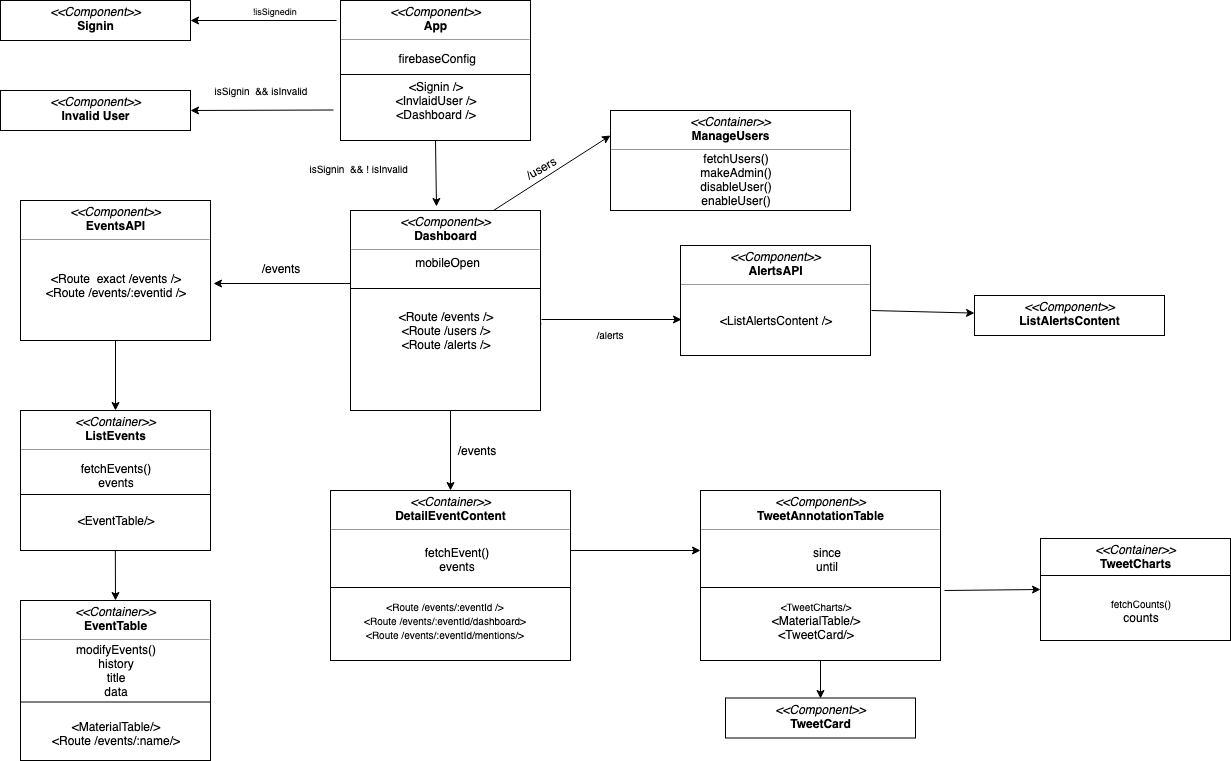
\includegraphics[width=150mm]{figs/front_diagram.png}
    \end{center}
\label{xfigDiagram}
\end{figure}


See Figure \ref{fig:frontdiag} for the class diagram depicting the redux states and actions and their associated react components. I have segregated components into two types:

\begin{itemize}
    \item \textbf{Containers}: Containers are react components that are connected to redux i.e. use the “connect” component from the react-router-dom package.
    \item \textbf{Components}: These are often referred to as dumb components or simply components. They render the data based on the properties that are passed from their containers.
\end{itemize}

Class diagrams are not exactly built for react-redux classes. We have modified the classical class diagram by adopting the following conventions:

\begin{itemize}
    \item The class can be a container or a component. This is depicted in the first line within the $<<$ $>>$ notation.
    \item Just below the same notation, we have the class name specified. 
    \item The first block contains the variables from mapStateToProps and mapDispatchToProps. we distinguish between the action and the state variable in the following way: we append parenthesis with action names and the state variables are retained as is.
\end{itemize}

\subsubsection{Authorization/Authentication}

Since most of the back-end systems of my infrastructure are Google products (Google cloud, Google storage, etc.), it only made sense to continue relying on Google for authentication. I started to look into Google Firebase for the security and authentication of the system. It provides me with React UI components out of the box, thereby reducing development time. For sign up and sign in, I decided to use Google as the authorization mechanism. Given that the University of Colorado Boulder provides a personal Google account to all students and affiliates, I know that any Project EPIC analyst will have access to a Google account. 

Once a login is performed, Firebase issues an OAuth 2.0 authorization in the form of a JWT token. This token can be modified from the back-end to include arbitrary key-value pairs. In this case, I use this storage to decide whether a user can access the application. A simple key is stored internally on demand to give access to a user. This is synchronized using Google Cloud Identity Platform and Firebase. 

To manage this part, I designed the Auth API. This service queries the Google Cloud Identity Platform to list any users that tried to sign in with a Google account. In addition, the service checks whether a user has the specific key-value in their authentication permissions. This is returned in the form of JSON. Another endpoint allows for any signed-in user with authorization to revoke or enable access for any other user. This is a simple approach to user control and can fail for a large group of users. However, Project EPIC does not have a large number of internal users.

For authorization, the front-end sends the JWT token with each request to an API. This token is checked from the API using a Java library specific to Project EPIC. If the token is invalid or it does not have a good key-value, then the service does not allow the operation to proceed and returns a non-authorized error. This authorization process is injected into the application using the DropWizard authorization library. In addition to simplifying the development of the APIs, the authorization library allows quick disabling through a simple boolean. This feature allows testing APIs without a valid token and then requiring the token when they are deployed in production.


